\section{NS3-FL:\ Bridging Data \&\ Network Management}
It has become clear to this point that one of the key insprations of this research study is to
introduce a user-friendly interface for federating any machine learning pipeliine in a unified
approch that considers diverse datasets, algorithmic implementations and network interaction.
Despite the great work being conducted in the field of federated learning by countless researchers,
the above venture is something that has yet to be prioritized by an industry leader to produce.

Nonetheless, the paper \emph{ns3-fl: Simulating Federated Learning with ns-3} by Ekaireb et al.\cite{ekairebNs3flSimulatingFederated2022} in 2022,
introduced an innovative approach in which studied the amalgamation of a PyTorch-based FL simulator (flsim) with a network simulator (ns-3) to produce
a unified simulation framework. In this section, we will discuss the architecture and methodology of the proposed framework, that consisted
the groundwork for the conjuction of our federated learning setup with a network simulator.

\subsection{Framework Overview}
% The aim of \emph{ns3-fl framework} is to simulate federated learning under practical networking conditions. 
\begin{figure}[H]
    \centering
    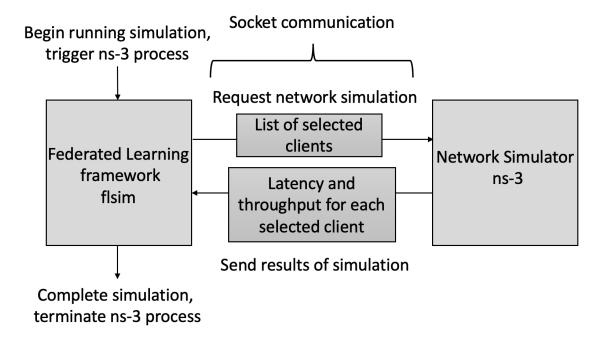
\includegraphics[width=0.8\textwidth]{figures/ns3-fl/ns3-fl_architecture.png}
    \caption{Architectural overview of ns3-fl. }
    \label{fig:architecture}
\end{figure}

\Cref{fig:architecture} depicts the top-level architecture of ns3-fl, that is decomposed in two software blocks in accordance with the previous description:
The FL framework of flsim for data distribution and FL processing, and the Ns3 Network simulator for network management and monitoring.

The depicted functionality can be summarized as follows: At the start of each FL training round, flsim initiates a network simulation request to ns-3,
specifying the selected clients. Ns-3 performs the network simulation and returns latency and throughput data for each client. Flsim, in turn, utilizes
these network statistics to calculate convergence time and average throughput for the training round.

\subsection{Learning, Network, and Power Models}
\subsubsection{Learning Model}
The learning model in ns3-fl supports both synchronous and asynchronous FL algorithms. The canonical settding is a star-topology network
(see \cref{sec:fl_topologies}) with $N$ client nodes connected to a central server. The learning process, represent a typical scneario of FL where
each client trains on its local dataset and sends model updates to the server. The objective is to minimize the overall loss function aggregated from all
clients' local losses. All the functions in regard with the learing process are processed by the flsim block.

\subsubsection{Network Model}
The network model in ns3-fl uses ns-3 to simulate realistic network conditions. Key metrics such as latency and throughput are considered
for each client. These metrics influence the overall convergence time and performance of the FL process. The framework supports various
network configurations, including wireless and ethernet connections.


\subsubsection{Power Model}
The power model calculates the energy consumption of FL training on client devices by modeling the consumption for two types of appliances:
Raspberry Pi (RPi) 4 and 400. In addition, to energy consumption, the time required for training for a specific device is calculated.
as the two elements are interconnected $E=P \cdot t$. For the computations the model takes into account machine-learning specific parameters such as the number
multiply–accumulate (MAC) operations, along with coeeficient parameters calculated by applying linear regression on the power measurements
for the two devices. This model helps in understanding the performance; including energy efficiency and time for training of different FL configurations.

\subsection{Implementation}
The implementation of ns3-fl involves creating Client and Server applications within ns-3, to mimic the data transmission conducted
for the global model distribution and the model updates. The communication between flsim and ns-3 is managed through the interprocess
communication protocol that is based on \emph{TCP Sockets}. The framework can be easily extended to include new data, algorithm, and
network models, as it is highly configurable through configuration files. \Cref{fig:workflow_ex} presents an example encompassing the
workflow during a complete training process. The communication between ns-3 and flsim is facilitated by four primary socket commands:
\begin{table}[H]
    \centering
    \begin{tabular}{|c|c|p{6cm}|}
        \hline
        \rowcolor{lightgray}
        \textbf{\#} & \textbf{Command} & \textbf{Use}                            \\
        \hline
        0           & RESPONSE         & Send results from ns-3 simulation       \\
        % \hline
        1           & STARTSIM         & Schedule a round simulation in ns-3     \\
        % \hline
        2           & EXIT             & Terminate ns-3 process                  \\
        % \hline
        3           & ENDSIM           & For async, alerts that ns-3 round ended \\
        \hline
    \end{tabular}
    \caption{Summary of socket commands used in ns3-fl.}
    \label{tab:socket_commands}
\end{table}

\begin{figure}[!ht]
    \centering
    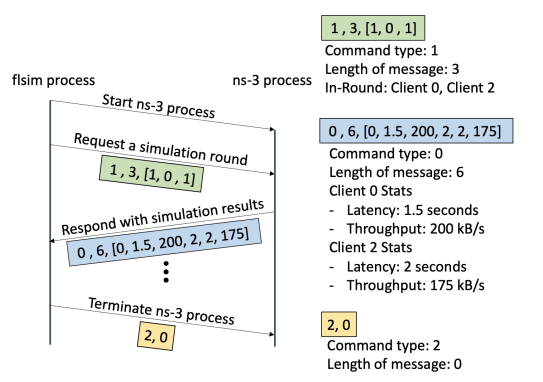
\includegraphics[width=.7\textwidth]{figures/ns3-fl/workflow_ex.png}
    \caption{Synchronous federated learning training workflow.}
    \label{fig:workflow_ex}
\end{figure}

Observing the flow diagram the FL simulator (flsim) after starting, initializes the network simulator (NS3).
Subsequently, to start a simulation for a training round a request is sent of $command type: 1$ including the list
of participating clients. Then NS3 runs a network simulation round using the selected set of participants. There
is a mapping between the two simulators in order to match their corresponding clients. When the round is complete,
a response is sent back to flsim containing the simulated latencies and throughput of the participants. That
way the interprocess communication is finalized for this communication round. This process is clearly depicted
in \cref{fig:workflow_ex} along with an explained example.


\subsection{Simulation Results}
The ns3-fl framework was validated through both a real deployment of Raspberry Pis and large-scale simulations.
The validation focused on measuring the framework's accuracy, training time, and energy consumption, comparing these
metrics against those obtained from the real deployment. The results demonstrated that ns3-fl accurately replicates
real-world federated learning scenarios, with errors not exceeding $1.5\%$. An illustration of the results is provided
in \cref{tab:ns3-fl_results}
For robustness, the analysis also included varying datasets, local epochs, and client selection strategies.

\begin{table}[H]
    \centering
    \begin{tabular}{|c|c|c|c|}
        \hline
        \rowcolor{lightgray}
        \textbf{Experiment} & \textbf{MNIST}     & \textbf{FashionMNIST} & \textbf{CIFAR-10}  \\
        \hline
        Real, RPi 400       & 18.32 $\pm$ 2.12   & 29.69 $\pm$ 1.10      & 33.86 $\pm$ 6.57   \\
        ns3-fl, RPi 400     & 20.55 $\pm$ 1.1E-5 & 27.78 $\pm$ 1.9E-5    & 30.44 $\pm$ 1.4E-5 \\
        \hline
        Real, RPi 4         & 18.91 $\pm$ 0.84   & 27.85 $\pm$ 1.17      & 30.30 $\pm$ 1.47   \\
        ns3-fl, RPi 4       & 19.01 $\pm$ 1.1E-5 & 27.44 $\pm$ 1.9E-5    & 30.15 $\pm$ 1.4E-5 \\
        \hline
    \end{tabular}
    \caption{Comparison of computational time (in seconds) between real deployment and ns3-fl simulations on different datasets.}
    \label{tab:ns3-fl_results}
\end{table}

Additionally, a series of simulations was conducted under different data distributions and network conditions to assess the
performance and scalability of various federated learning configurations. These simulations provided valuable insights into
how different setups affect the overall efficiency and scalability of federated learning systems.

\subsection{Conclusion}
The ns3-fl framework provides a compelling tool for simulating federated learning under realistic network conditions.
By integrating flsim with ns-3, researchers can validate their FL algorithms considering the interplay between data,
algorithm, and network. The framework's ability to accurately replicate real-world scenarios makes it a valuable resource
for advancing federated learning research, as well as, a great starting base for implementing novel approaches in unifing
network and data management, similar to the one described in our thesis.
